\begin{enumerate}
\item $ABC$ is a right triangle in which $\angle B = 90\degree$. If $AB = 8 cm$ and $BC = 6 cm$, find the diameter of the circle inscribed in the triangle.

\item Draw two concentric circles of radii $2 cm$ and $5 cm$. Take a point $P$ on the outer circle and construct a pair of tangents $PA$ and $PB$ to the smaller circle. Measure $PA$.  


\item In  \figref{fig:Figh_3}, $PQ$ and $RS$ are two parallel tangents to a circle with centre $O$ and another tangent $AB$ with point of contact $C$ intersecting $PQ$ at $A$ and $RS$ at $B$. Prove that $\angle AOB = 90 \degree$
\begin{figure}[H]
    \centering
    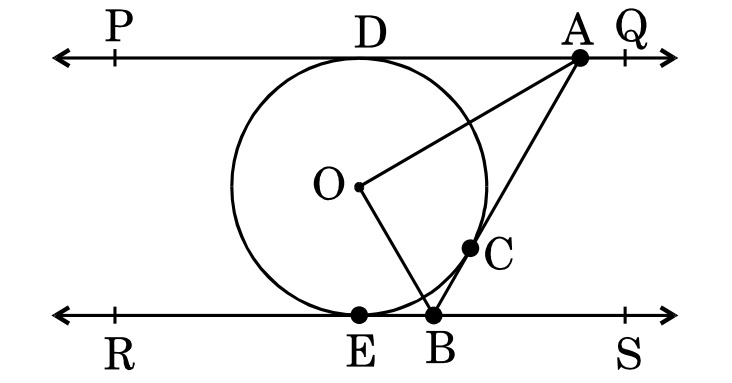
\includegraphics[width=\columnwidth]{figs/img3.jpg}
    \caption{Tangent and Circle}
    \label{fig:Figh_3}
\end{figure}
\end{enumerate}
